% Transient stability assessment of the IEEE 39-bus system with an SVM
% Compile with pdflatex (Overleaf, MiKTeX or TeX Live). Figures are read from ./figures/.
\documentclass[11pt,a4paper]{article}

\usepackage[T1]{fontenc}
\usepackage[utf8]{inputenc}
\usepackage{lmodern}
\usepackage[margin=2.4cm]{geometry}
\usepackage{graphicx}
\usepackage{booktabs}
\usepackage{array}
\usepackage{float}
\usepackage[font=small,labelfont=bf]{caption}
\usepackage{amsmath,amssymb}
\usepackage{xcolor}
\usepackage{listings}
\usepackage[hidelinks]{hyperref}

\graphicspath{{figures/}}

\definecolor{codebg}{HTML}{F7F7F5}
\definecolor{codekw}{HTML}{256ABF}
\definecolor{codecomment}{HTML}{6B6A66}
\definecolor{codestring}{HTML}{B8302F}
\lstdefinestyle{py}{
  language=Python,
  basicstyle=\ttfamily\footnotesize,
  keywordstyle=\color{codekw}\bfseries,
  commentstyle=\color{codecomment}\itshape,
  stringstyle=\color{codestring},
  backgroundcolor=\color{codebg},
  frame=single, rulecolor=\color{black!15},
  breaklines=true, columns=fullflexible, keepspaces=true,
  showstringspaces=false,
  numbers=left, numberstyle=\tiny\color{codecomment},
  xleftmargin=1.8em, framexleftmargin=1.8em,
  captionpos=b, aboveskip=0.8em, belowskip=0.8em
}
\lstset{style=py}

\newcommand{\code}[1]{\texttt{#1}}

\title{\textbf{Transient Stability Assessment of the\\IEEE 39-Bus System Using a Support Vector Machine}\\[0.4em]
\large First experiment: all simulated cases, outliers retained}
\author{Project group} % TODO: add names, registration numbers and supervisor
\date{\today}

\begin{document}
\maketitle

\begin{abstract}
\noindent
Fast transient stability assessment lets operators react to a disturbance before the system loses synchronism.
This report trains a Support Vector Machine (SVM) to predict whether the IEEE 39-bus system stays stable after a
contingency, using only four voltage-magnitude and four frequency samples measured at each of the ten generator buses
(80 inputs). The dataset contains 3\,715 simulated cases: generator trips, line trips, ground faults followed by line
tripping, and load disconnections, each at five load levels and, for faults, three fault durations. The stability
label comes from the transient stability index (TSI); 18.2\,\% of the cases are unstable.
In this first experiment all cases are used and the physically impossible readings are kept in the training data.
The data are split \emph{by contingency} into training, validation and test sets (about 70/15/15) so that no
contingency is seen in more than one set. The SVM settings are chosen by grouped five-fold cross-validation inside
the training set, which selects robust scaling with $C = 10$ and $\gamma = 0.001$ (balanced accuracy
$0.974 \pm 0.016$). The model reaches a balanced accuracy of 0.961 on the validation set and 0.955 on the untouched
test set, where it finds 93 of 97 unstable cases (95.9\,\%) with an ROC-AUC of 0.992. Of the 25 test errors, 21 are false
alarms, and ten of these come from just two contingencies; one of them, the trip of the generator at Bus~38, produces
frequencies outside the range seen in training.
\end{abstract}

\tableofcontents
\newpage

%=====================================================================================
\section{Introduction}
%=====================================================================================
Transient stability is the ability of a power system to keep its synchronous generators in step after a large
disturbance such as a fault, the loss of a line or the loss of a generator. Time-domain simulation gives an exact
answer but is too slow for real-time use when many contingencies must be screened. Machine-learning classifiers
trained on simulated cases can give an answer within milliseconds from a few post-disturbance measurements.

\paragraph{Objective.} Build a classifier that takes the voltage and frequency measured at the ten generator buses
(B30--B39) of the IEEE 39-bus system at four post-disturbance sampling instants and predicts whether the case is
\emph{stable} or \emph{unstable}.

\paragraph{Scope of this report.} This is the first experiment: all simulated cases are used and the physically
impossible readings produced by large fluctuations are kept. The report describes the dataset, an exploratory
analysis, the modelling procedure (data split, preprocessing, SVM, hyperparameter selection and evaluation), the
results, and the software that implements them. Section~\ref{sec:future} lists the changes planned for later
experiments.

%=====================================================================================
\section{Dataset}
%=====================================================================================
\subsection{Simulated scenarios}
The dataset (\code{IEEE39\_voltage\_frequency\_4sample\_SVM\_dataset.csv}) was produced by time-domain simulation of
the IEEE 39-bus (New England) system. % TODO: name the simulation tool and the sampling instants of samples 1-4
Four contingency types were simulated (Table~\ref{tab:scenarios}). Every contingency was run at five operating
conditions in which the system load is changed by $-4$, $-2$, 0, $+2$ and $+4$\,\%. Ground faults were applied at
20\,\% and 80\,\% of the line length, as single-line-to-ground (SLG), double-line-to-ground (LLG) or three-phase-to-ground
(3PHG) faults, and cleared after 0.1, 0.3 or 0.5\,s by tripping the line. Line trips use the same three durations.
All 34 transmission lines are covered.

\begin{table}[htbp]
\centering
\caption{Contingencies in the dataset. Every contingency appears once at each of the five load levels.}
\label{tab:scenarios}
\begin{tabular}{lrrrr}
\toprule
Contingency type & Contingencies & Cases & Unstable & Unstable (\%) \\
\midrule
Generator trip                  & 10  & 50     & 5   & 10.0 \\
Ground fault + line trip        & 612 & 3\,060 & 458 & 15.0 \\
\quad SLG                       & 204 & 1\,020 & 30  & 2.9 \\
\quad LLG                       & 204 & 1\,020 & 72  & 7.1 \\
\quad 3PHG                      & 204 & 1\,020 & 356 & 34.9 \\
Line trip                       & 102 & 510    & 213 & 41.8 \\
Load disconnection              & 19  & 95     & 0   & 0.0 \\
\midrule
Total                           & 743 & 3\,715 & 676 & 18.2 \\
\bottomrule
\end{tabular}
\end{table}

\subsection{Model inputs}
For each generator bus B30--B39 the dataset holds four samples of the voltage magnitude (p.u.) and four samples of
the frequency (Hz), giving $10 \times (4+4) = 80$ inputs (Table~\ref{tab:features}). Only these 80 measurements are
given to the model; the scenario descriptors (contingency type, load level, fault duration) are used for analysis only,
because a real-time assessment tool would not know them in this form.

\begin{table}[htbp]
\centering
\caption{Input features.}
\label{tab:features}
\begin{tabular}{lll}
\toprule
Quantity & Column names & Count \\
\midrule
Voltage magnitude (p.u.) & \code{B30\_Vmag\_1} \dots\ \code{B39\_Vmag\_4}     & 40 \\
Frequency (Hz)           & \code{B30\_FreqHz\_1} \dots\ \code{B39\_FreqHz\_4} & 40 \\
\midrule
Total & & 80 \\
\bottomrule
\end{tabular}
\end{table}

\subsection{Stability label}
The label \code{Overall\_Stability} was derived from the transient stability index (TSI). A widely used definition is
\begin{equation}
  \mathrm{TSI} = \frac{360^\circ - \Delta\delta_{\max}}{360^\circ + \Delta\delta_{\max}} \times 100,
  \label{eq:tsi}
\end{equation}
where $\Delta\delta_{\max}$ is the largest rotor-angle separation between any two generators during the simulation.
A case is labelled \textbf{stable (1)} when $\mathrm{TSI} > 0$ and \textbf{unstable (0)} otherwise.
% TODO: confirm that Eq. (1) matches the TSI definition used in the simulations
The dataset contains 3\,039 stable cases (81.8\,\%) and 676 unstable cases (18.2\,\%).

\subsection{Data quality}
Table~\ref{tab:quality} summarises the checks. There are no missing values, infinite values or duplicate rows.
Ten rows contain physically impossible readings: voltages of 9--13\,p.u.\ at B34 and frequencies between 24 and
81\,Hz at B33 and B34. All ten are three-phase faults on line 16--19 at 80\,\% of the line length, cleared after 0.3
or 0.5\,s (two contingencies, each at all five load levels), and all are labelled unstable. They arise from the large
fluctuations of the generators that lose synchronism. As planned for this first experiment, \textbf{these rows are
kept}, and they are used for training (Section~\ref{sec:split}).

\begin{table}[htbp]
\centering
\caption{Data-quality checks on the raw dataset.}
\label{tab:quality}
\begin{tabular}{lr}
\toprule
Check & Count \\
\midrule
Rows / columns                              & 3\,715 / 85 \\
Missing values                              & 0 \\
Infinite values                             & 0 \\
Duplicate rows                              & 0 \\
Rows with a voltage above 1.1 p.u.          & 10 \\
Rows with $|f - 50\,\mathrm{Hz}| > 5$\,Hz   & 10 \\
Rows with any impossible reading            & 10 \\
\bottomrule
\end{tabular}
\end{table}

%=====================================================================================
\section{Exploratory analysis}
%=====================================================================================
\subsection{Class balance}
Only about one case in five is unstable (Figure~\ref{fig:balance}). A model that always answered ``stable'' would
already be 81.8\,\% accurate, so plain accuracy is a poor yardstick. The model therefore uses class weights, and the
results are reported mainly as balanced accuracy and the recall of the unstable class (Section~\ref{sec:metrics}).

\begin{figure}[htbp]
  \centering
  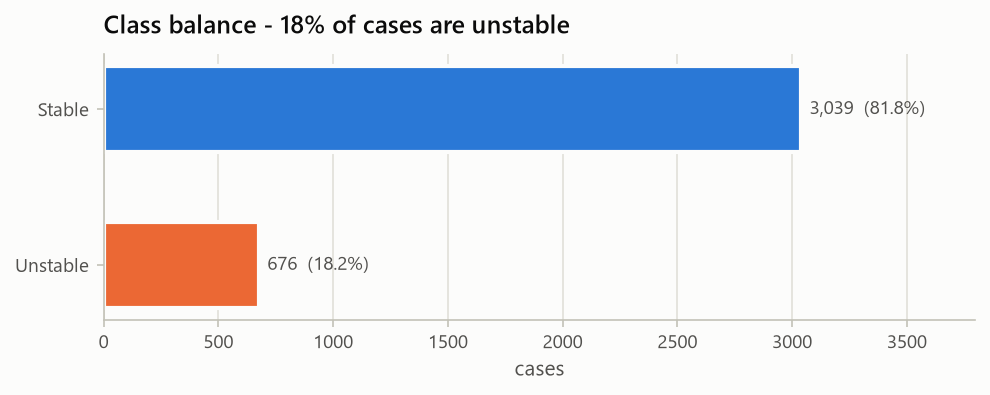
\includegraphics[width=0.8\linewidth]{01_class_balance.png}
  \caption{Number of stable and unstable cases.}
  \label{fig:balance}
\end{figure}

\subsection{What makes a case unstable?}
Line trips are the most often unstable contingency (41.8\,\%), followed by ground faults (15.0\,\%) and generator
trips (10.0\,\%, only the trip of the Bus~39 unit); load disconnections are always stable (Figure~\ref{fig:bytype}).

\begin{figure}[htbp]
  \centering
  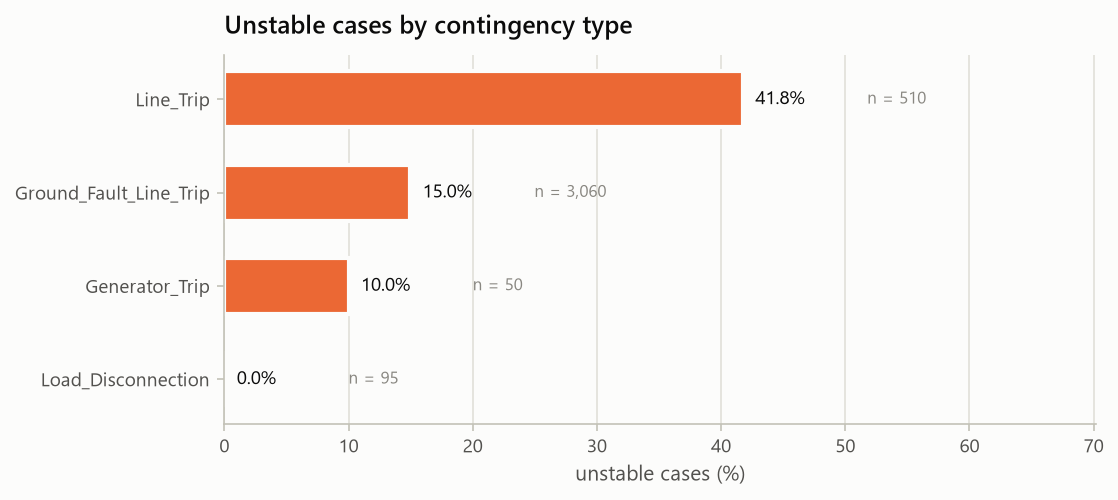
\includegraphics[width=0.8\linewidth]{02_unstable_by_contingency_type.png}
  \caption{Share of unstable cases per contingency type ($n$ = number of cases).}
  \label{fig:bytype}
\end{figure}

Fault duration is the strongest driver (Figure~\ref{fig:faulttime}). With 0.1\,s clearing, only 2.9\,\% of the
cases are unstable for every fault kind; at 0.5\,s, 68.8\,\% of three-phase faults and 78.2\,\% of line trips are
unstable. Three-phase faults are far more severe than LLG faults, which are more severe than SLG faults.
The fault location (20\,\% or 80\,\% of the line) hardly matters (15.2\,\% versus 14.8\,\% unstable).

The 2.9\,\% unstable at 0.1\,s are exactly the contingencies on \textbf{line 16--19}: all 105 cases on this line are
unstable. Tripping it disconnects buses 19, 20, 33 and 34, and with them the generators at B33 and B34, from the rest
of the network.

\begin{figure}[htbp]
  \centering
  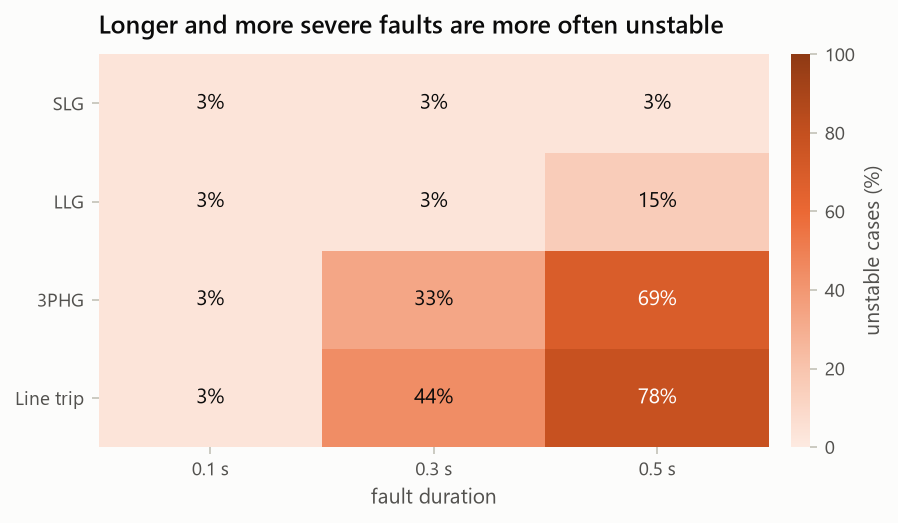
\includegraphics[width=0.62\linewidth]{03_unstable_by_fault_and_time.png}
  \caption{Share of unstable cases by fault kind and fault duration.}
  \label{fig:faulttime}
\end{figure}

A heavier load makes line trips and ground faults more often unstable (Figure~\ref{fig:load}); overall the unstable
share rises from 13.9\,\% at $-4$\,\% load to 22.5\,\% at $+4$\,\%. Of the 743 contingencies, 576 are stable at every
load level, 103 are unstable at every load level and 64 change label with the load. All 64 change in the physically
expected direction: stable at light load, unstable at heavy load.

\begin{figure}[htbp]
  \centering
  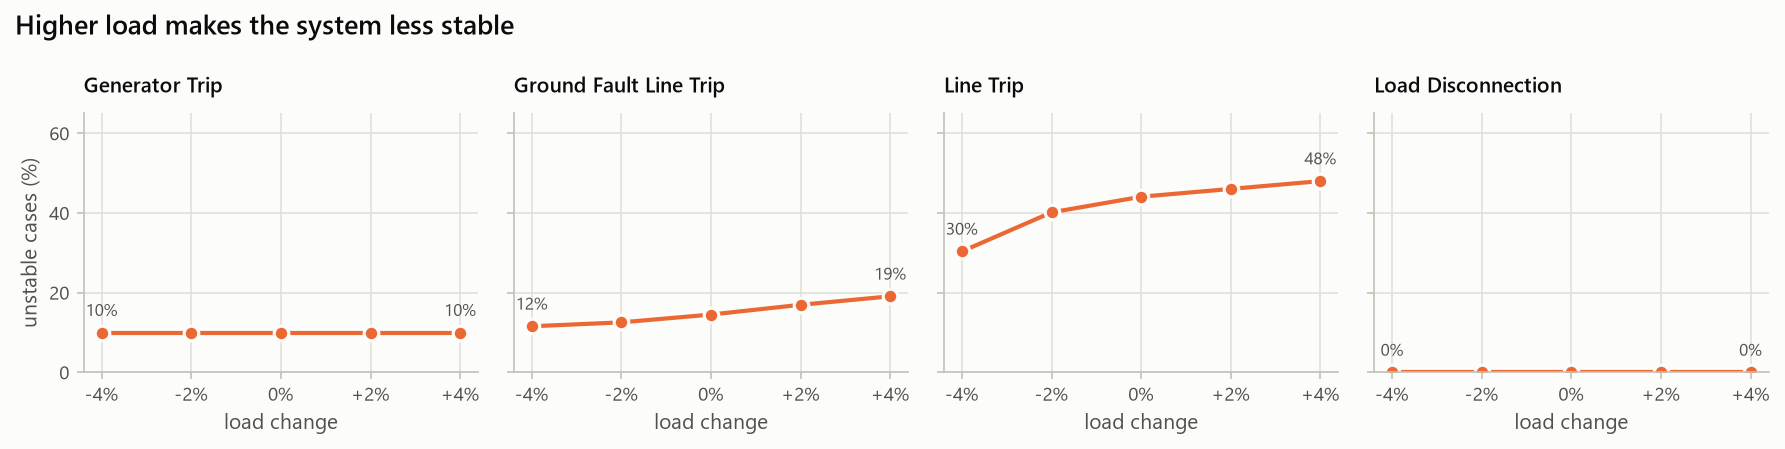
\includegraphics[width=\linewidth]{04_unstable_vs_load.png}
  \caption{Share of unstable cases against the load change, per contingency type.}
  \label{fig:load}
\end{figure}

\subsection{Voltage and frequency behaviour}
Figures~\ref{fig:vtrace} and~\ref{fig:ftrace} show the median and the middle 50\,\% of each measurement over the four
samples. Unstable cases have clearly lower generator voltages, with the largest gaps at B31 and B32, and higher,
more widely spread frequencies (over-frequency), again most visible at B31 and B32. B39 differs least between the
classes, and B38 differs mainly in frequency. B31 operates at about 0.7--0.8\,p.u.\ even in stable cases.

\begin{figure}[htbp]
  \centering
  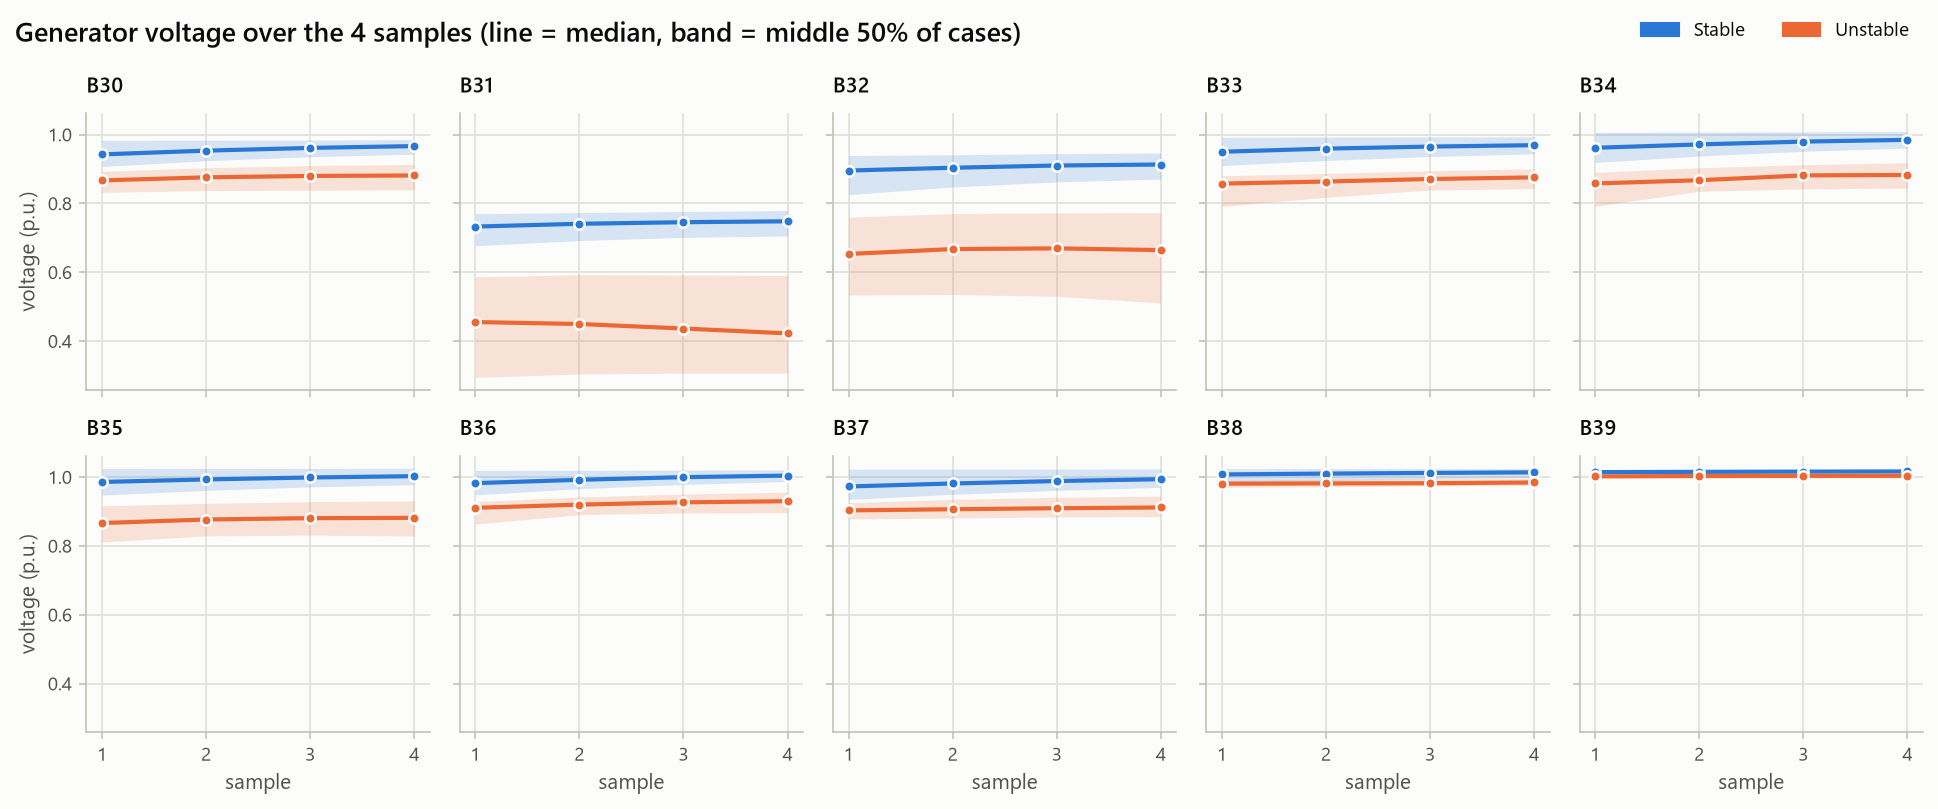
\includegraphics[width=\linewidth]{05_voltage_traces.png}
  \caption{Generator voltage magnitude over the four samples. Line: median; band: interquartile range.}
  \label{fig:vtrace}
\end{figure}

\begin{figure}[htbp]
  \centering
  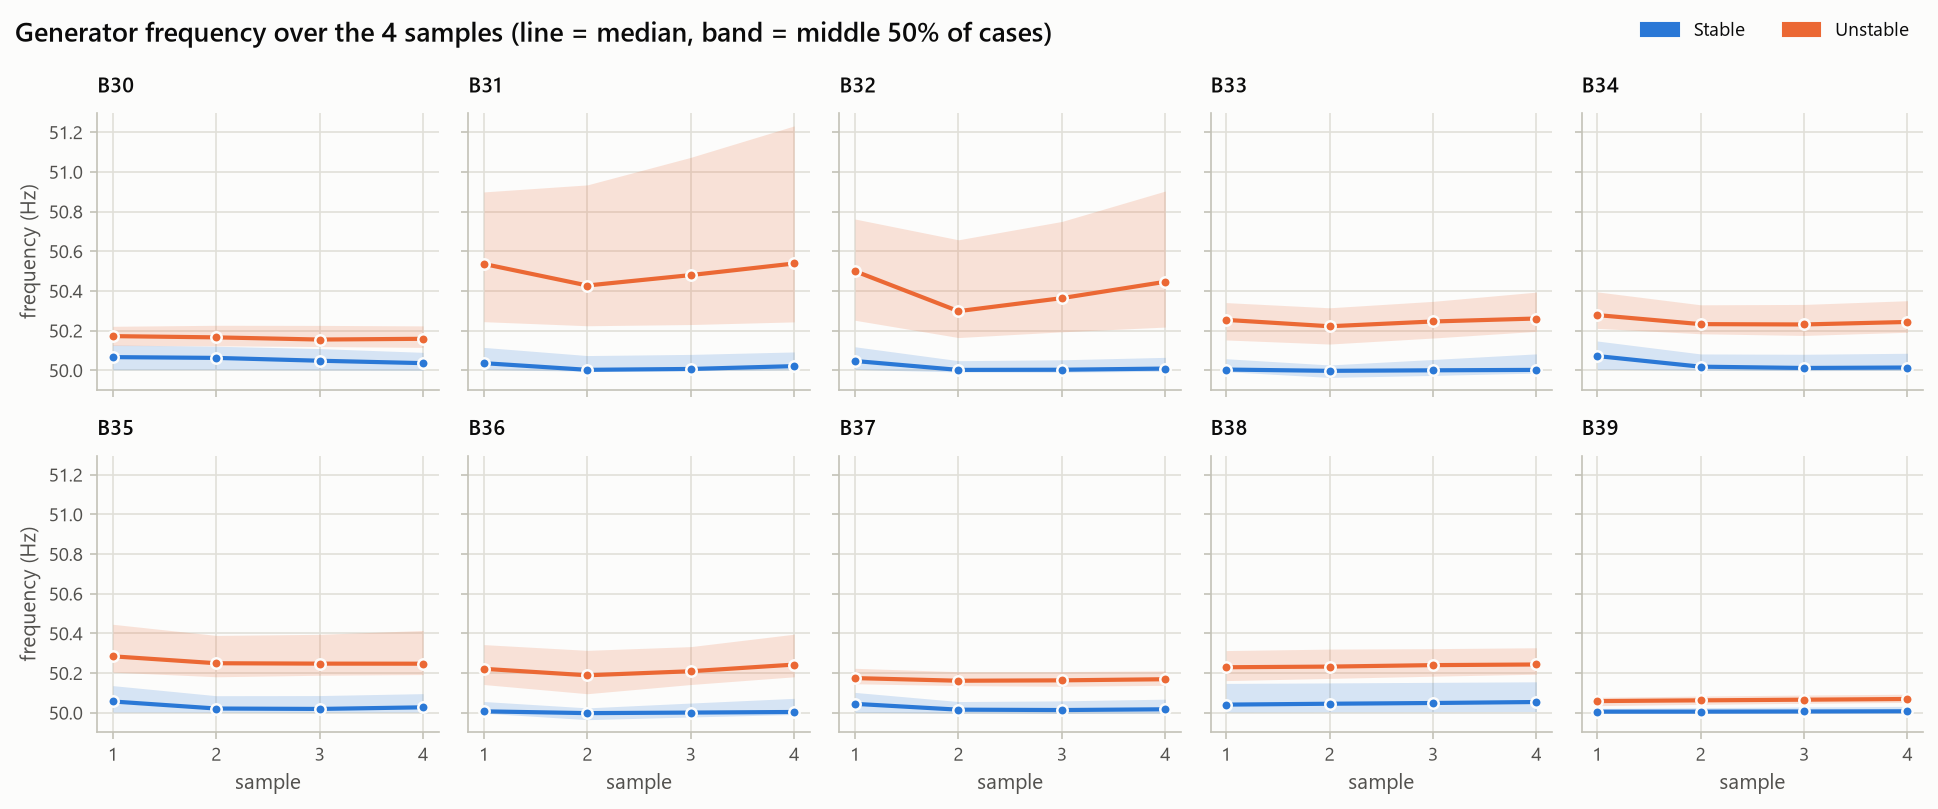
\includegraphics[width=\linewidth]{06_frequency_traces.png}
  \caption{Generator frequency over the four samples. Line: median; band: interquartile range.}
  \label{fig:ftrace}
\end{figure}

Figure~\ref{fig:extreme} shows, for every case, the largest voltage and the largest frequency deviation (logarithmic
scale). The ten impossible readings stand far above all others. Apart from them, unstable cases typically deviate by
0.1--4\,Hz and stable cases by less than 1\,Hz.

\begin{figure}[htbp]
  \centering
  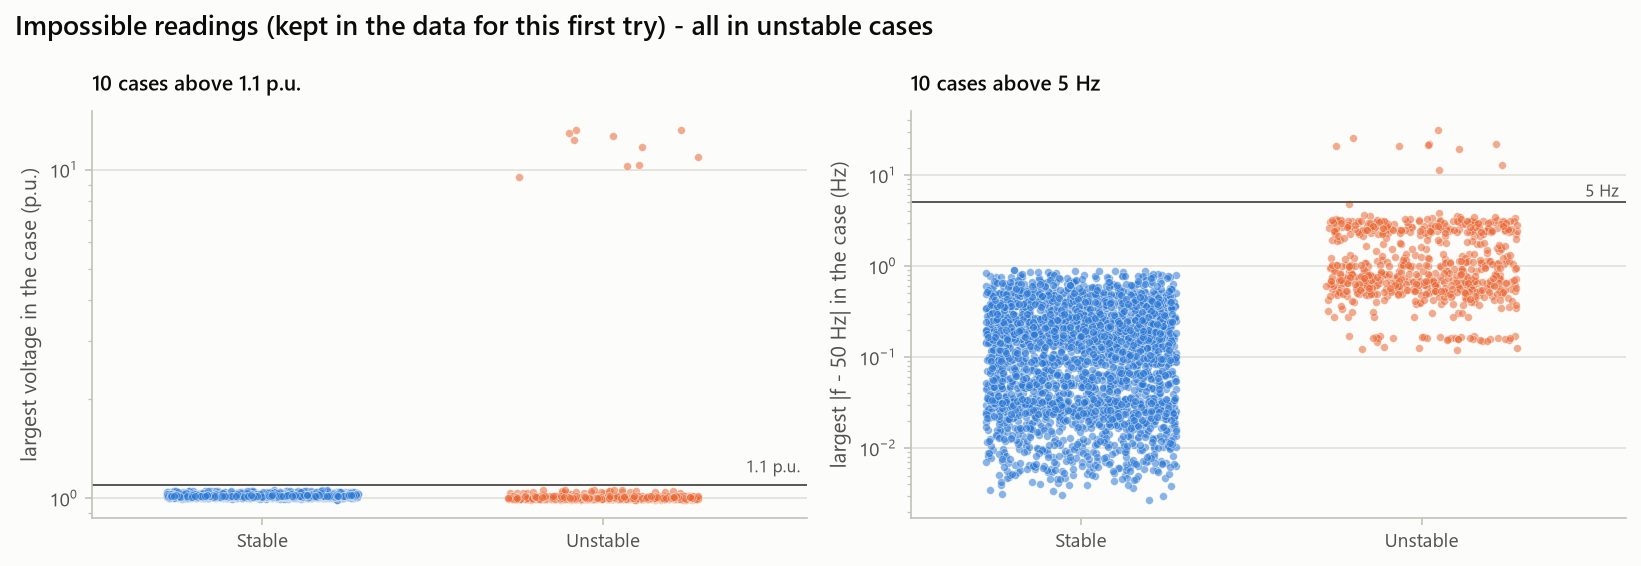
\includegraphics[width=\linewidth]{07_impossible_readings.png}
  \caption{Largest voltage (left) and largest frequency deviation (right) of each case. Points above the line are
  physically impossible; they are kept in this experiment.}
  \label{fig:extreme}
\end{figure}

\subsection{Redundancy and separability}
The four samples of the same bus are strongly correlated (bright $4\times4$ blocks on the diagonal of
Figure~\ref{fig:corr}), so the 80 inputs carry much less than 80 independent pieces of information. A two-dimensional
principal-component projection (Figure~\ref{fig:pca}) already places many unstable cases away from the stable
cluster, while the remainder overlap it. Separating those requires all 80 dimensions and a non-linear boundary, which
motivates the RBF-kernel SVM.

\begin{figure}[htbp]
  \centering
  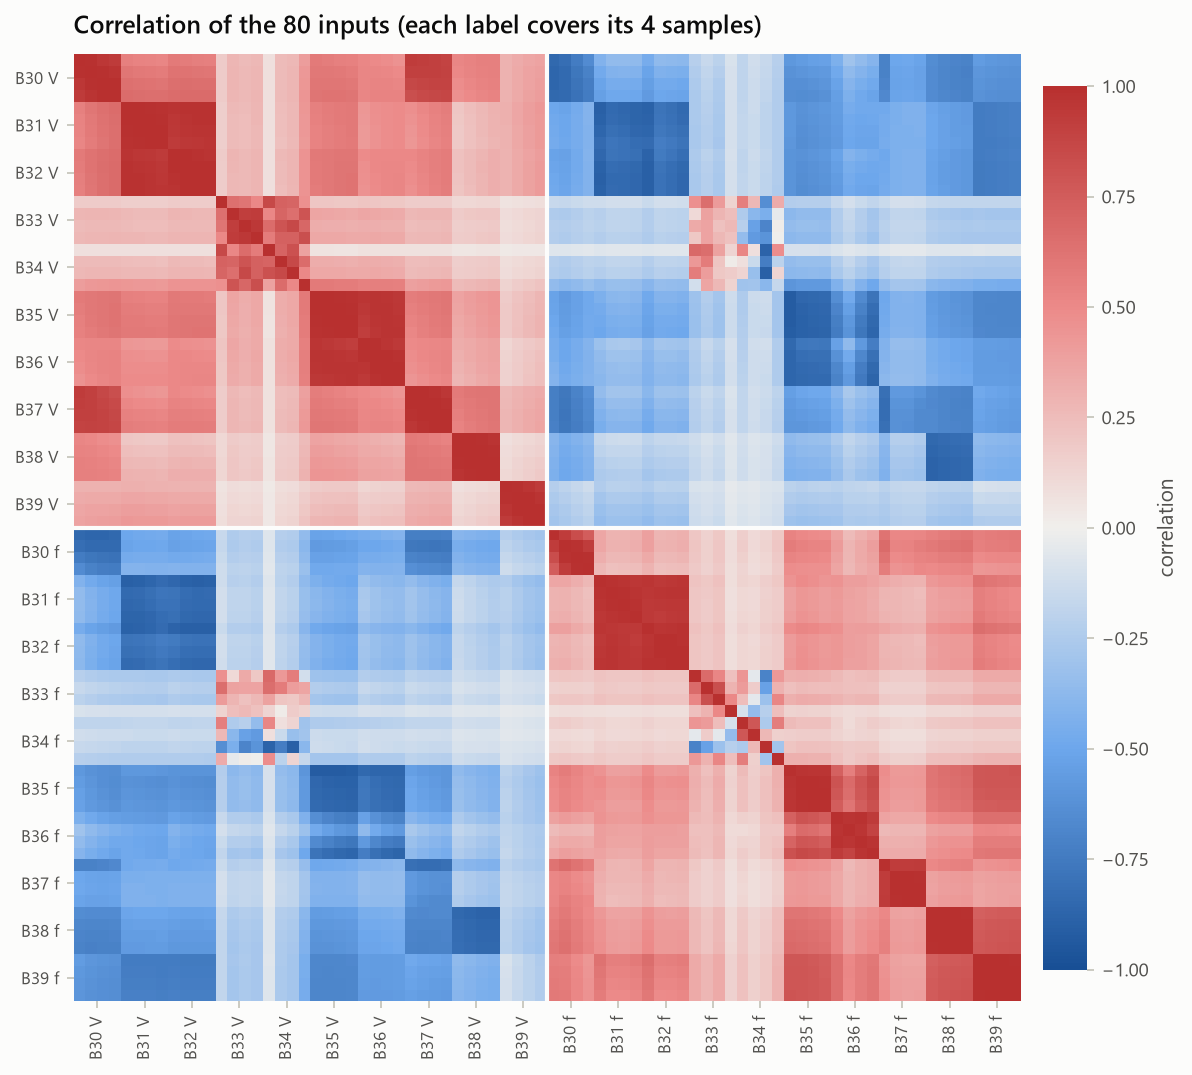
\includegraphics[width=0.78\linewidth]{08_correlation.png}
  \caption{Correlation matrix of the 80 inputs (labels mark the four samples of each bus; V = voltage, f = frequency).}
  \label{fig:corr}
\end{figure}

\begin{figure}[htbp]
  \centering
  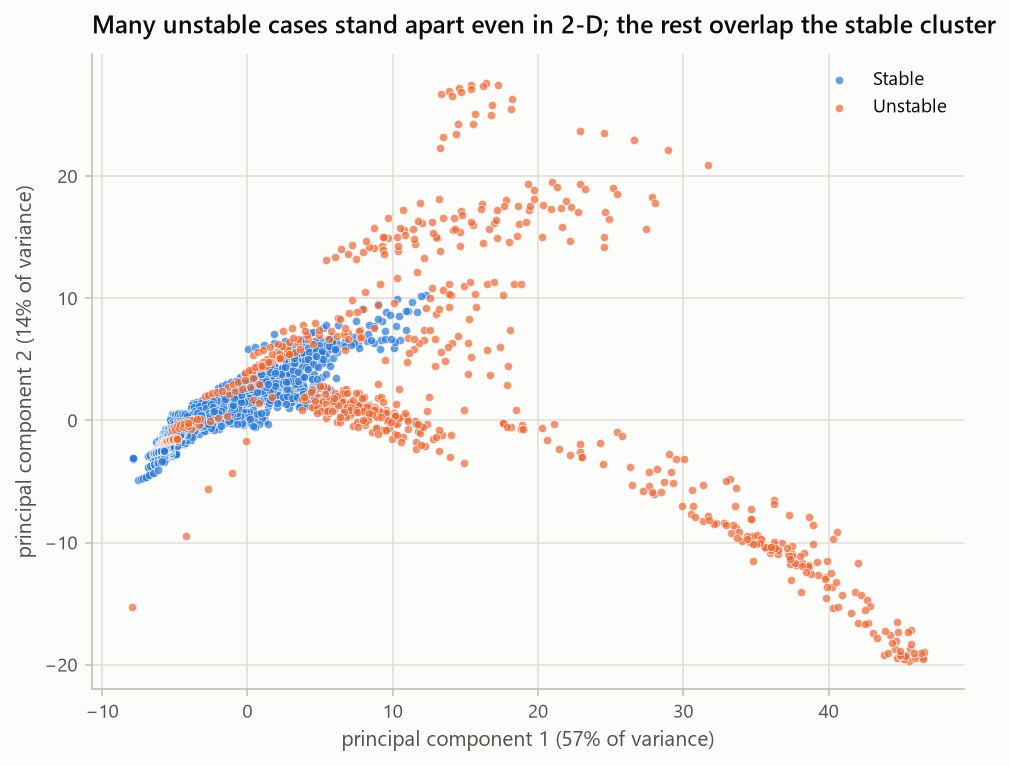
\includegraphics[width=0.7\linewidth]{09_pca.png}
  \caption{Projection of all cases on the first two principal components (after robust scaling).}
  \label{fig:pca}
\end{figure}

%=====================================================================================
\section{Methodology}
%=====================================================================================
\subsection{Procedure}
\begin{enumerate}
  \item Load all 3\,715 cases; nothing is removed.
  \item Split the cases \emph{by contingency} into training, validation and test sets (about 70/15/15).
  \item Choose the scaler and the SVM hyperparameters $C$ and $\gamma$ by grouped five-fold cross-validation
        inside the training set.
  \item Fit the chosen model on the training set and check it on the validation set.
  \item Refit the chosen model on training + validation data and evaluate it \emph{once} on the test set.
  \item Analyse the errors and the feature importance; save the model for prediction of new cases.
\end{enumerate}

\subsection{Training, validation and test split}
\label{sec:split}
Each contingency appears five times (once per load level), and the five cases are very similar. If the rows were
split at random, near-identical cases would land in both training and test sets and the test score would overstate
how well the model handles a contingency it has never seen. The split is therefore made by
\code{Contingency\_ID}: all five load levels of a contingency go to the same set. A stratified group split
(\code{StratifiedGroupKFold}) keeps the share of unstable cases equal in the three sets (Table~\ref{tab:split},
Figure~\ref{fig:split}). No contingency is shared between any two sets.

The two contingencies that contain the impossible readings are always assigned to the \textbf{training} set. This
experiment is meant to train \emph{with} these readings, and a later experiment that removes or caps them can then be
compared on exactly the same validation and test sets. All ten impossible rows are therefore in the training set and
none in the validation or test sets.

\begin{table}[htbp]
\centering
\caption{Training, validation and test sets.}
\label{tab:split}
\begin{tabular}{lrrrrrr}
\toprule
Set & Cases & Share (\%) & Contingencies & Stable & Unstable & Unstable (\%) \\
\midrule
Training   & 2\,655 & 71.5 & 531 & 2\,172 & 483 & 18.2 \\
Validation & 530    & 14.3 & 106 & 434    & 96  & 18.1 \\
Test       & 530    & 14.3 & 106 & 433    & 97  & 18.3 \\
\bottomrule
\end{tabular}
\end{table}

\begin{figure}[htbp]
  \centering
  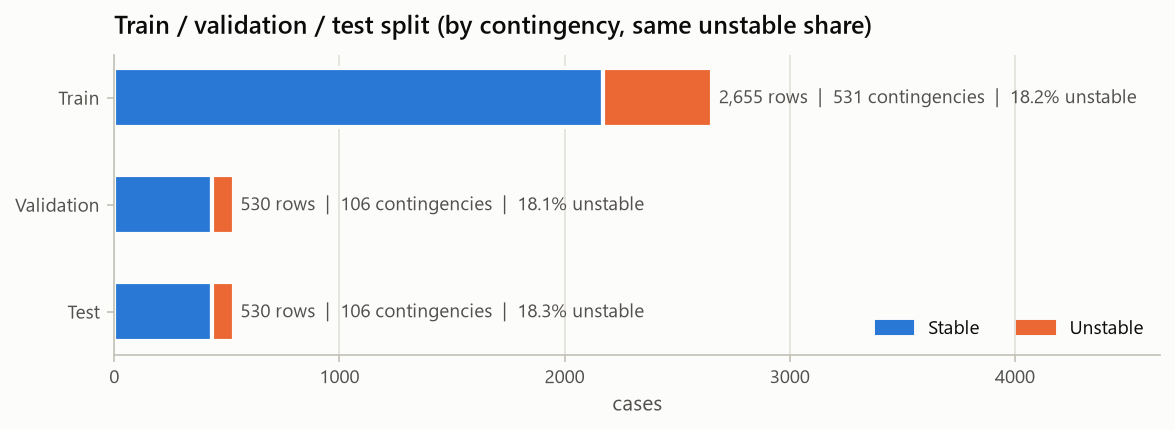
\includegraphics[width=0.9\linewidth]{10_split.png}
  \caption{Composition of the three sets.}
  \label{fig:split}
\end{figure}

\subsection{Support Vector Machine}
For training cases $(\mathbf{x}_i, y_i)$ with $y_i = +1$ (stable) or $-1$ (unstable), the soft-margin SVM solves
\begin{equation}
  \min_{\mathbf{w},\, b,\, \boldsymbol{\xi}} \;\; \frac{1}{2}\lVert \mathbf{w} \rVert^2
  + C \sum_{i} c_{y_i}\, \xi_i
  \quad \text{s.t.} \quad y_i\bigl(\mathbf{w}^\top \phi(\mathbf{x}_i) + b\bigr) \ge 1 - \xi_i,\;\; \xi_i \ge 0,
\end{equation}
where $C$ sets how strongly training errors are penalised and $\phi$ maps the inputs into a feature space defined by
the radial basis function (RBF) kernel
\begin{equation}
  K(\mathbf{x}, \mathbf{x}') = \exp\!\left(-\gamma\, \lVert \mathbf{x} - \mathbf{x}' \rVert^2\right).
\end{equation}
A large $\gamma$ makes each training case influence only its close neighbourhood (a more flexible boundary).
The class weights $c_k = n / (2 n_k)$ (``balanced'') compensate for the class imbalance: in the training set an error
on an unstable case costs about 4.5 times more than an error on a stable case. The trained classifier is
\begin{equation}
  f(\mathbf{x}) = \sum_{i \in \mathrm{SV}} \alpha_i y_i K(\mathbf{x}_i, \mathbf{x}) + b,
\end{equation}
and this report uses the \textbf{instability score} $s(\mathbf{x}) = -f(\mathbf{x})$: a case is predicted unstable when
$s(\mathbf{x}) > 0$, and the larger $|s|$, the further the case lies from the decision boundary.

\subsection{Preprocessing}
The inputs have different units and ranges, so they are scaled before the SVM. Two scalers were compared; the
scaling parameters are always learned from the training data only (both are steps of one scikit-learn
\code{Pipeline}).
\begin{itemize}
  \item \textbf{Standard:} $z_j = (x_j - \mu_j)/\sigma_j$.
  \item \textbf{Robust + clip:} $z_j = \operatorname{clip}\bigl((x_j - \mathrm{median}_j)/\mathrm{IQR}_j,\,-20,\,20\bigr)$.
        The median and interquartile range are not distorted by the impossible readings, and clipping stops such
        readings from dominating the kernel distance. No rows are removed.
\end{itemize}

\subsection{Hyperparameter selection}
\label{sec:tuning}
The grid in Table~\ref{tab:grid} (60 combinations) was evaluated by \textbf{grouped five-fold cross-validation inside
the training set}: the 531 training contingencies are divided into five groups, each group is held out once, and
the five balanced accuracies are averaged. The combination with the highest mean was chosen.

\begin{table}[htbp]
\centering
\caption{Hyperparameter grid.}
\label{tab:grid}
\begin{tabular}{ll}
\toprule
Parameter & Values \\
\midrule
Scaler   & standard, robust + clip \\
$C$      & 0.1, 1, 10, 100, 1000 \\
$\gamma$ & \code{scale} $= 1/(80\,\mathrm{Var}(\mathbf{z}))$, 0.001, 0.003, 0.01, 0.03, 0.1 \\
Kernel / class weight & RBF / balanced (fixed) \\
\bottomrule
\end{tabular}
\end{table}

\paragraph{Why not choose on the validation set alone?} The validation set holds only 106 contingencies, about 20 of
them unstable, so one validation score is noisy. Scoring the same grid on the validation set alone
(Figure~\ref{fig:valgrid}) would pick robust scaling with $C = 1000$, $\gamma = 0.03$ (validation balanced accuracy
0.993), but this setting reaches only 0.967 in cross-validation, below the chosen setting. During development, with an
earlier version of the split, the validation-only favourite even scored 0.923 in cross-validation against 0.969 for
the cross-validated choice. The settings are therefore chosen by cross-validation, and the validation set serves as an
independent check before the test set is used.

\subsection{Evaluation metrics}
\label{sec:metrics}
The unstable class is treated as the positive class. With TP (unstable predicted unstable), FN (unstable predicted
stable), FP (stable predicted unstable) and TN (stable predicted stable):
\begin{align}
  \text{Unstable recall} &= \frac{TP}{TP + FN}, &
  \text{Stable recall} &= \frac{TN}{TN + FP}, \\
  \text{Balanced accuracy} &= \tfrac{1}{2}\left(\frac{TP}{TP + FN} + \frac{TN}{TN + FP}\right), &
  \text{Unstable precision} &= \frac{TP}{TP + FP}.
\end{align}
A missed unstable case (FN) is the costly error in operation; a false alarm (FP) only triggers an unnecessary check.
The ROC-AUC and the average precision measure how well the instability score ranks unstable above stable cases,
independently of the decision threshold.

%=====================================================================================
\section{Results}
%=====================================================================================
\subsection{Selected model}
Cross-validation (Figure~\ref{fig:cvgrid}, Table~\ref{tab:cvtop} in Appendix~\ref{app:grid}) selects
\textbf{robust scaling + clipping with $C = 10$ and $\gamma = 0.001$}, with a cross-validated balanced accuracy of
$\mathbf{0.974 \pm 0.016}$. The best standard-scaler setting ($C = 100$, $\gamma = 0.001$) reaches $0.972 \pm 0.013$,
so the difference between the scalers is small and within the spread between folds. Very small $C$ underfits
(balanced accuracy 0.91--0.94 at $C = 0.1$), and very large $\gamma$ also lowers the score.

\begin{figure}[htbp]
  \centering
  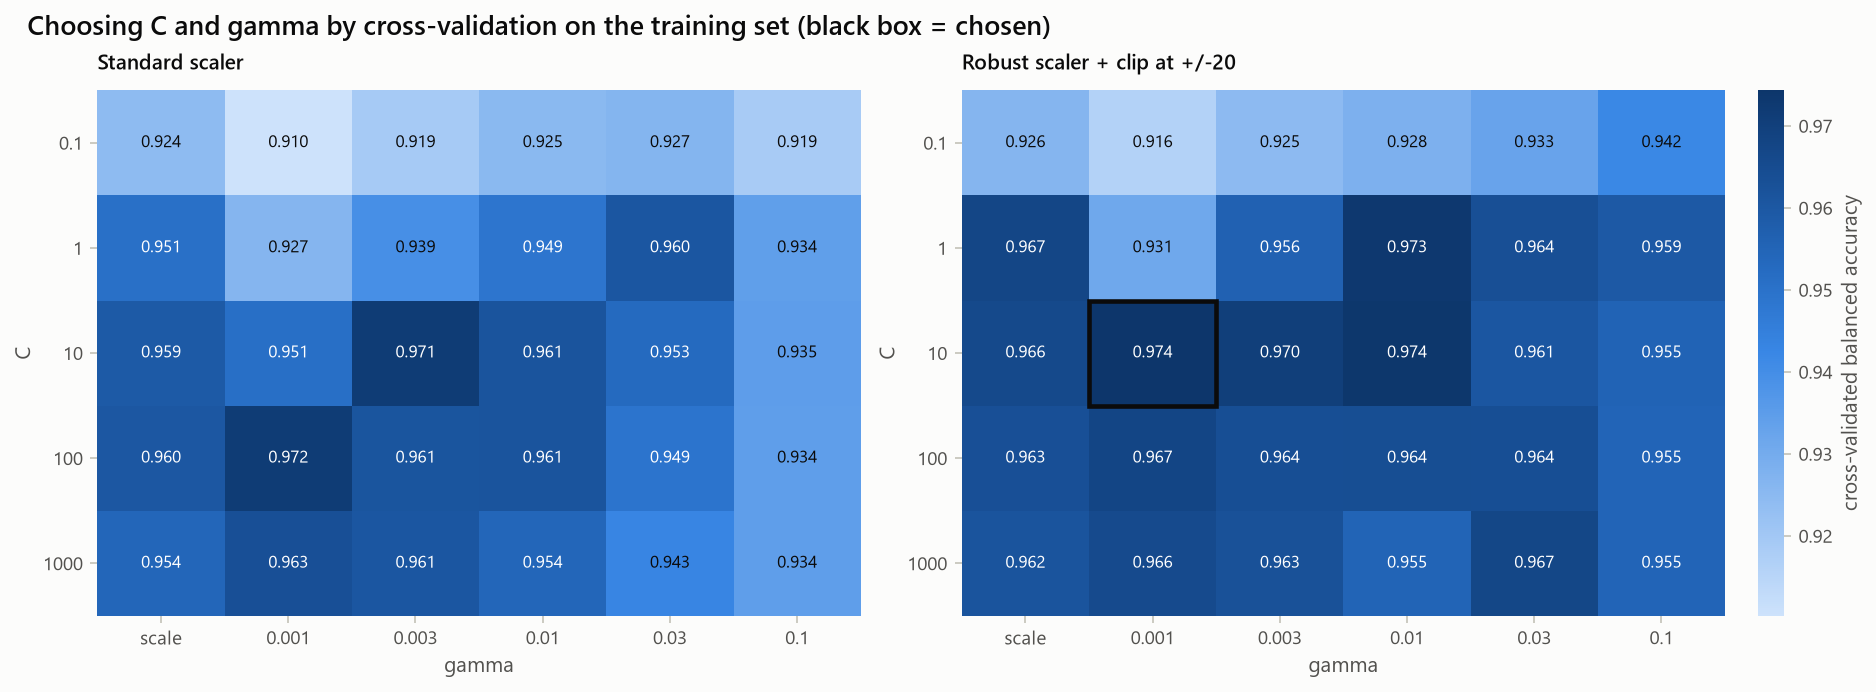
\includegraphics[width=\linewidth]{11_cv_grid.png}
  \caption{Cross-validated balanced accuracy for every combination; the black box marks the chosen setting.}
  \label{fig:cvgrid}
\end{figure}

\begin{figure}[htbp]
  \centering
  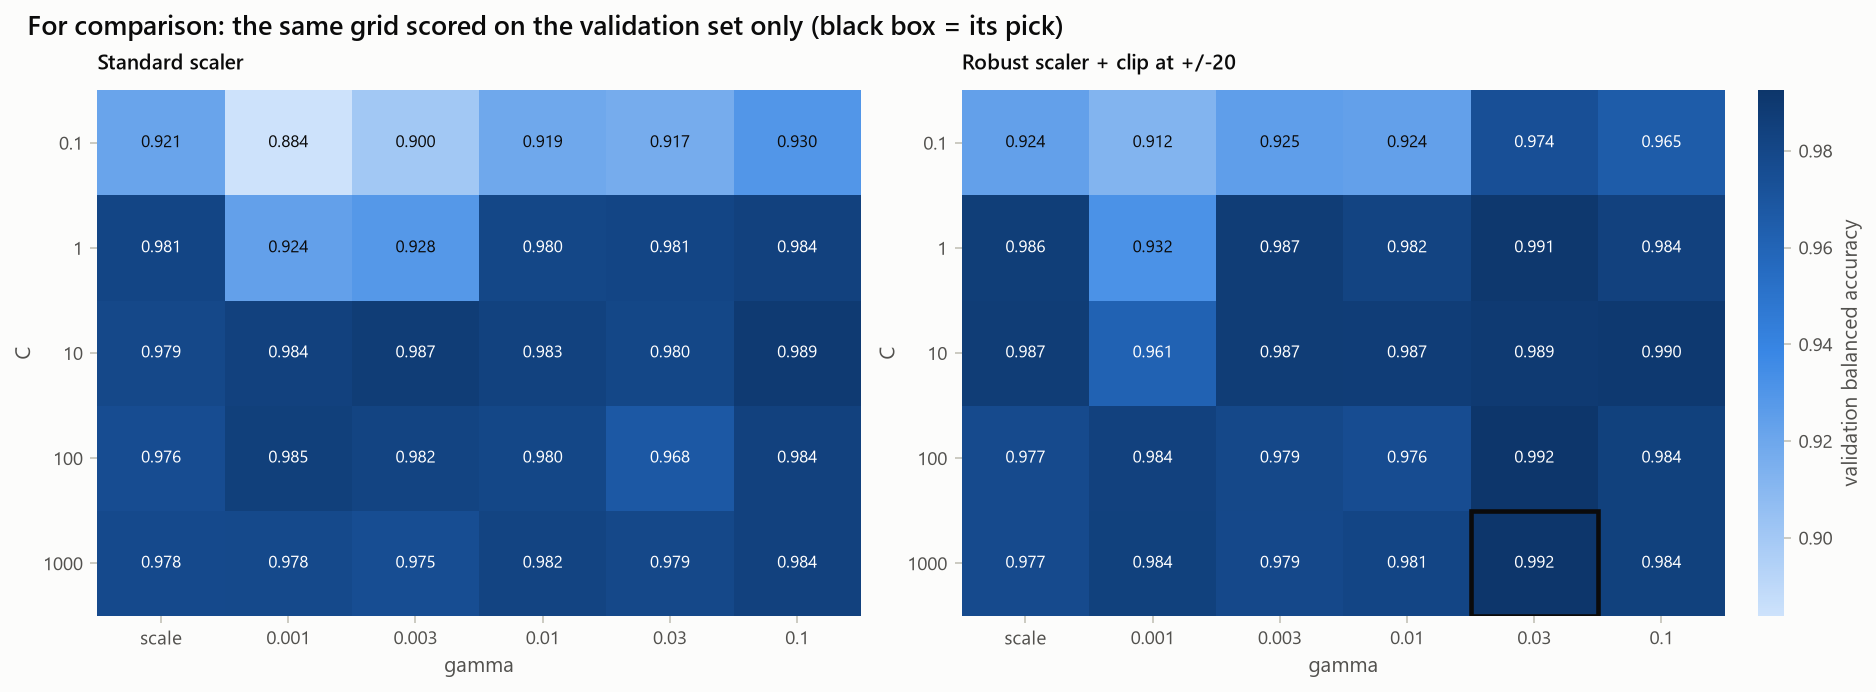
\includegraphics[width=\linewidth]{12_validation_only_grid.png}
  \caption{For comparison: the same grid scored on the validation set only. Its preferred setting differs from the
  cross-validated choice and scores lower (0.967) in cross-validation.}
  \label{fig:valgrid}
\end{figure}

\subsection{Validation check}
Fitted on the training set, the selected model reaches a balanced accuracy of 0.961 on the validation set; it finds
91 of 96 unstable cases and raises 11 false alarms among 434 stable cases (Table~\ref{tab:results},
Figure~\ref{fig:cm}). The 16 errors come from only 9 contingencies, because a contingency that is hard for the model
is usually hard at several load levels:
\begin{itemize}
  \item all five missed unstable cases are one contingency, a three-phase fault on line 16--19 at 80\,\% cleared after
        0.1\,s. The fault is short, so the four samples show only small deviations, yet the loss of line 16--19
        always ends unstable;
  \item a three-phase fault on line 16--17 at 20\,\% cleared after 0.3\,s (3 false alarms) and the trip of line
        4--14 after 0.3\,s (2 false alarms);
  \item six single false alarms on severe (0.3--0.5\,s) faults close to the stability boundary.
\end{itemize}

\paragraph{Learning curve.} Training on 10\,\% to 100\,\% of the training contingencies (Figure~\ref{fig:lc}) raises
the validation balanced accuracy from 0.87--0.92 with up to 1\,060 training cases to 0.96--0.97 with 1\,600 cases or
more, after which it levels off. The training score stays at 0.975--0.985. With the current kinds of scenarios the
model is close to its limit; further gains need more \emph{diverse} scenarios (for example more generator trips) rather
than more of the same.

\begin{figure}[htbp]
  \centering
  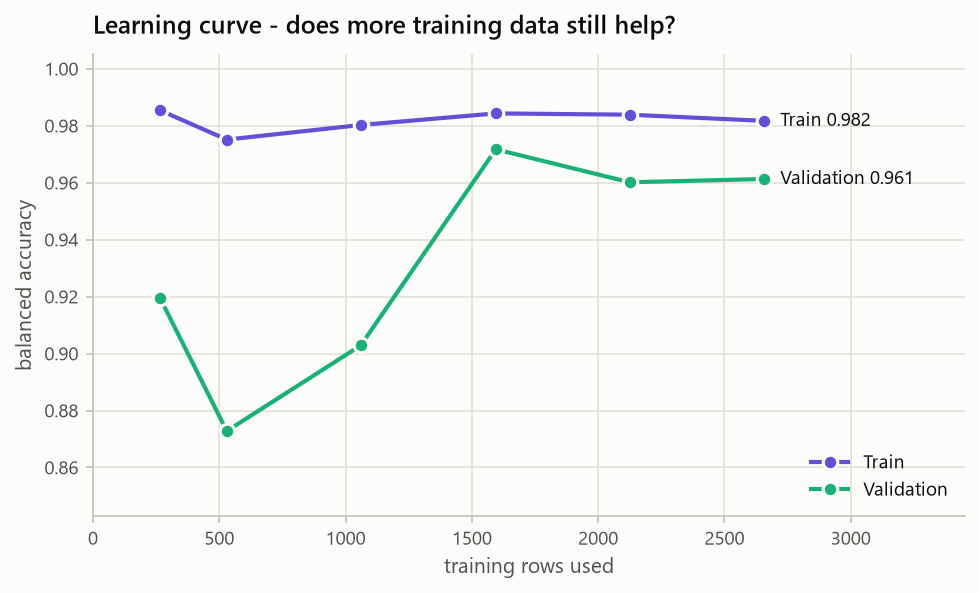
\includegraphics[width=0.75\linewidth]{13_learning_curve.png}
  \caption{Balanced accuracy on the training subset and on the validation set against the number of training cases.}
  \label{fig:lc}
\end{figure}

\subsection{Test results}
The chosen setting was refitted on the training and validation sets together (3\,185 cases) and evaluated once on
the 530 test cases. Table~\ref{tab:results} and Figure~\ref{fig:metrics} compare the three sets.

\begin{table}[htbp]
\centering
\caption{Results. Training and validation: model fitted on the training set. Test: final model fitted on training +
validation data.}
\label{tab:results}
\begin{tabular}{lrrrrrrr}
\toprule
Set & Accuracy & \shortstack{Balanced\\accuracy} & \shortstack{Unstable\\recall} & \shortstack{Unstable\\precision} &
\shortstack{Stable\\recall} & ROC-AUC & \shortstack{Average\\precision} \\
\midrule
Training   & 0.977 & 0.982 & 0.990 & 0.894 & 0.974 & 0.998 & 0.992 \\
Validation & 0.970 & 0.961 & 0.948 & 0.892 & 0.975 & 0.994 & 0.979 \\
Test       & \textbf{0.953} & \textbf{0.955} & \textbf{0.959} & \textbf{0.816} & \textbf{0.952} & \textbf{0.992} & \textbf{0.964} \\
\midrule
\multicolumn{8}{l}{Grouped 5-fold cross-validation on the training set: balanced accuracy $0.974 \pm 0.016$} \\
\bottomrule
\end{tabular}
\end{table}

\begin{figure}[htbp]
  \centering
  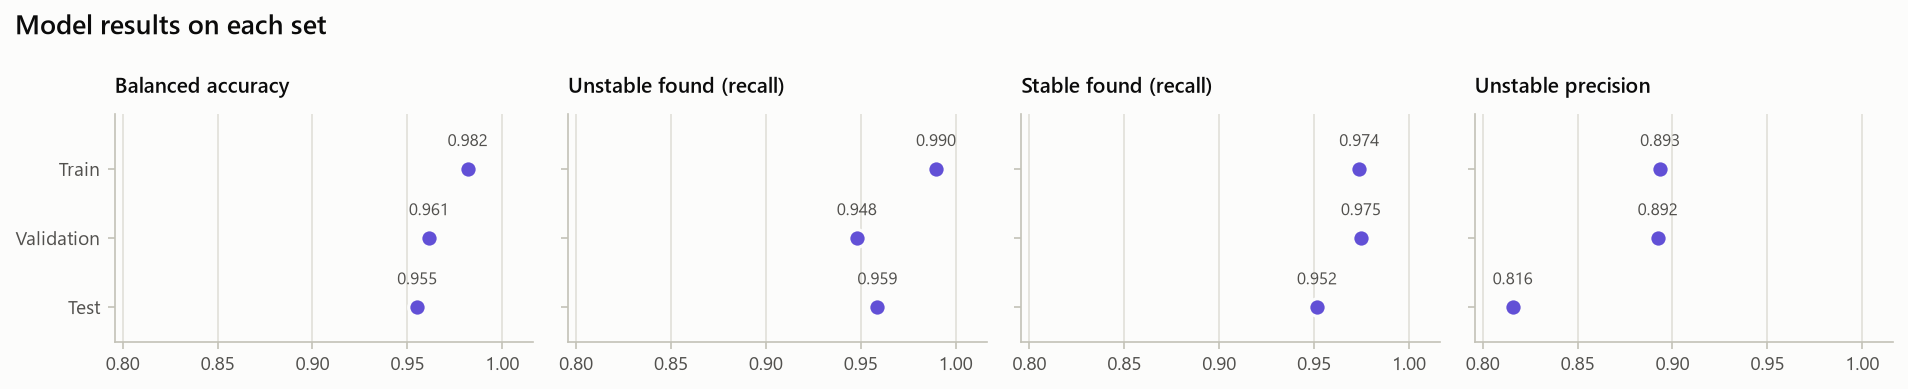
\includegraphics[width=\linewidth]{14_metrics_by_set.png}
  \caption{Main metrics on the training, validation and test sets.}
  \label{fig:metrics}
\end{figure}

On the test set the model finds \textbf{93 of 97 unstable cases} and wrongly flags 21 of 433 stable cases
(Figure~\ref{fig:cm}). The ROC and precision--recall curves (Figure~\ref{fig:roc}) show that the instability score ranks
unstable above stable cases very well (ROC-AUC 0.992, average precision 0.964). In the score distribution
(Figure~\ref{fig:score}) most stable cases have negative and most unstable cases positive scores. The four missed
unstable cases lie just below the boundary (scores $-0.15$ to $-0.05$).

\begin{figure}[htbp]
  \centering
  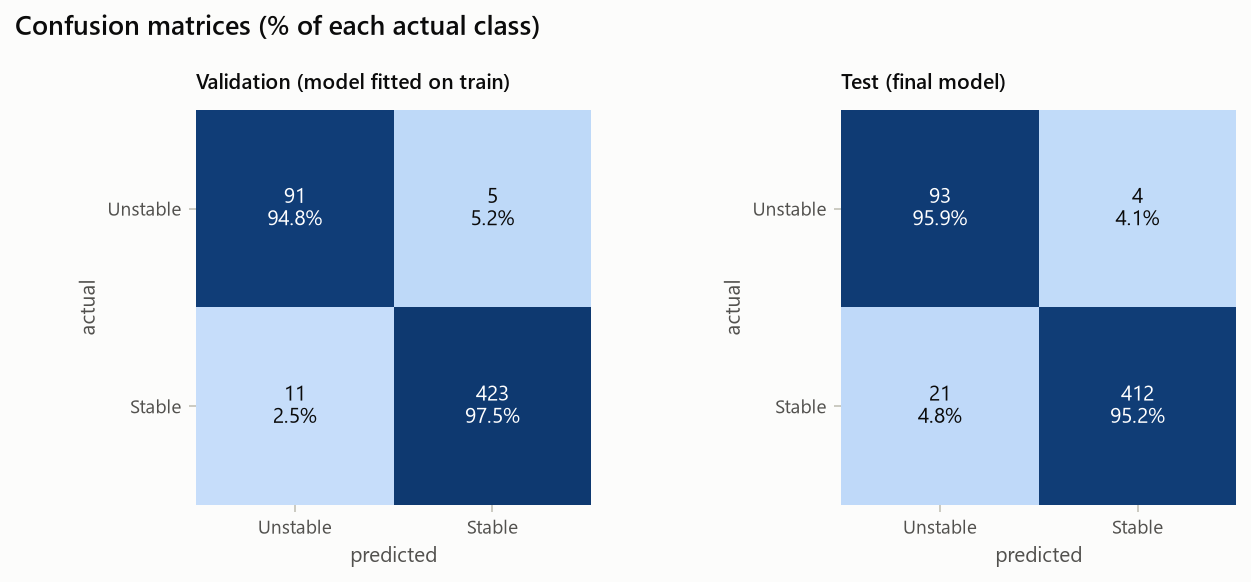
\includegraphics[width=0.85\linewidth]{15_confusion_matrices.png}
  \caption{Confusion matrices for the validation and test sets (count and share of each actual class).}
  \label{fig:cm}
\end{figure}

\begin{figure}[htbp]
  \centering
  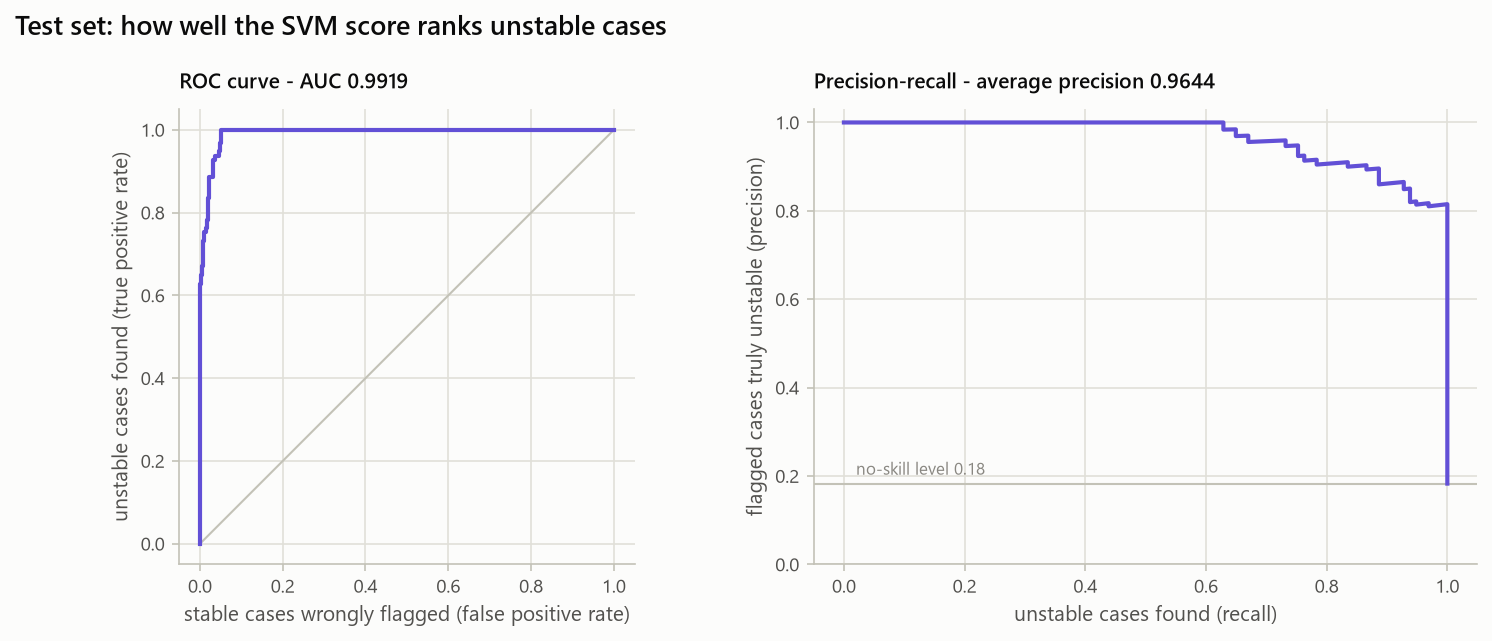
\includegraphics[width=\linewidth]{16_roc_pr_test.png}
  \caption{ROC curve (left) and precision--recall curve (right) on the test set, unstable as the positive class.}
  \label{fig:roc}
\end{figure}

\begin{figure}[htbp]
  \centering
  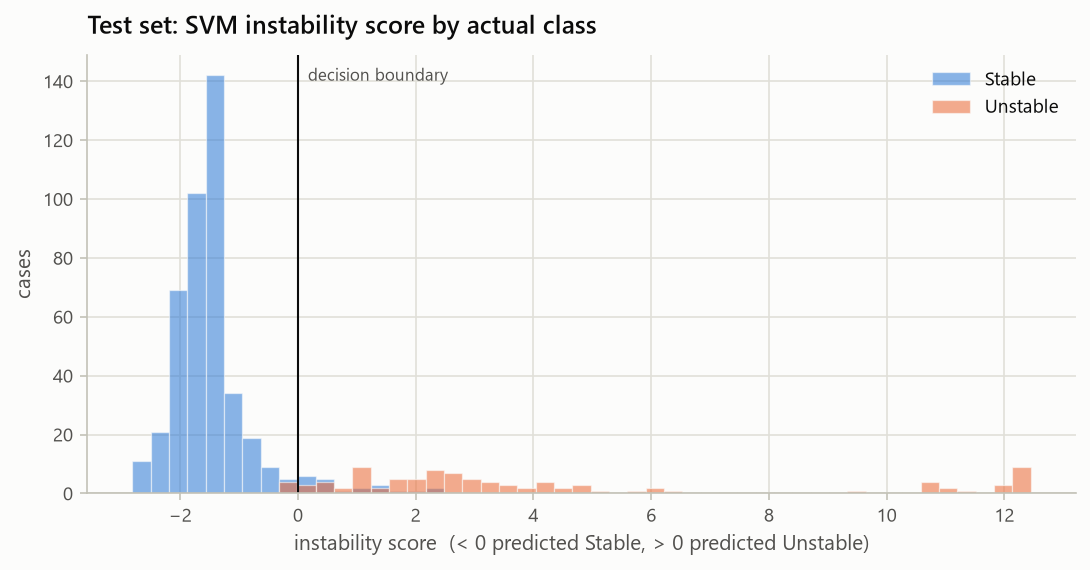
\includegraphics[width=0.85\linewidth]{17_score_distribution_test.png}
  \caption{Instability score of the test cases by actual class; cases right of the line are predicted unstable.}
  \label{fig:score}
\end{figure}

Per contingency type (Table~\ref{tab:bytype}, Figure~\ref{fig:bytypetest}), load disconnections are classified without
error, ground faults with 97.2\,\% accuracy and line trips with 90.0\,\%. The only generator trip in the test set, the
trip of the generator at Bus~38, is wrongly flagged as unstable at all five load levels. Accuracy lies between 94.3 and
97.2\,\% at every load level.

\begin{table}[htbp]
\centering
\caption{Test results per contingency type.}
\label{tab:bytype}
\begin{tabular}{lrrrrr}
\toprule
Contingency type & Cases & Accuracy & Unstable & Missed unstable & False alarms \\
\midrule
Generator trip           & 5   & 0.000 & 0  & 0 & 5 \\
Ground fault + line trip & 435 & 0.972 & 64 & 4 & 8 \\
Line trip                & 80  & 0.900 & 33 & 0 & 8 \\
Load disconnection       & 10  & 1.000 & 0  & 0 & 0 \\
\bottomrule
\end{tabular}
\end{table}

\begin{figure}[htbp]
  \centering
  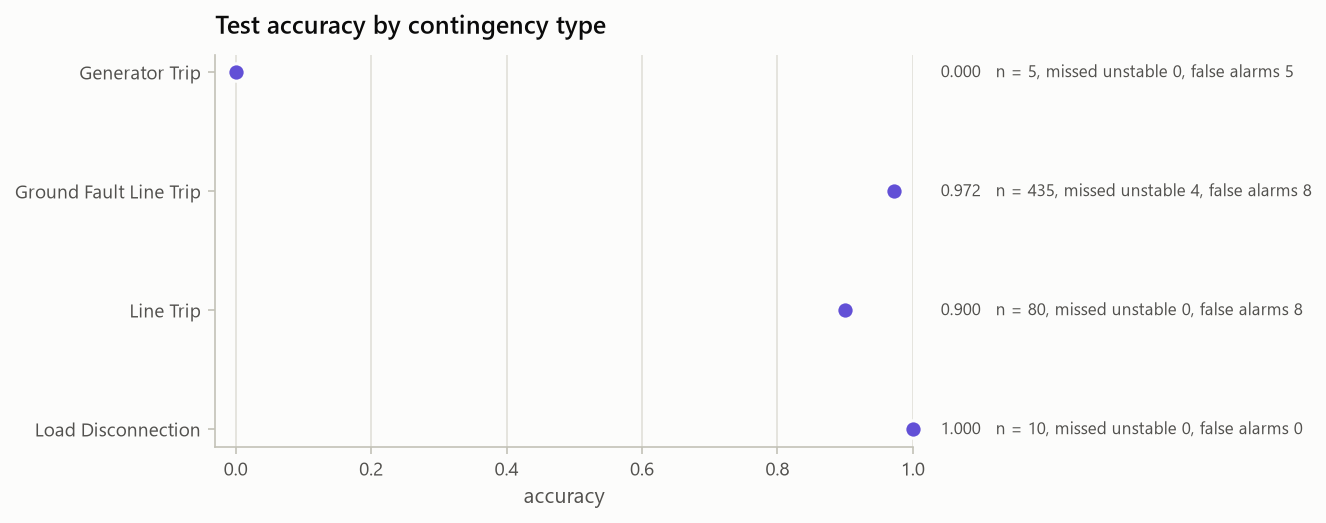
\includegraphics[width=0.85\linewidth]{18_test_by_contingency_type.png}
  \caption{Test accuracy per contingency type.}
  \label{fig:bytypetest}
\end{figure}

Table~\ref{tab:testerrors} groups the 25 test errors by contingency. Ten of the 21 false alarms come from just two
contingencies, each wrong at all five load levels:
\begin{itemize}
  \item \textbf{Trip of the generator at Bus~38.} After this trip the B38 frequency falls as low as 49.92\,Hz, below
        every case the final model was trained on (lowest 49.977\,Hz). The model is therefore extrapolating; the
        prediction tool flags these inputs as outside the training range. Only nine generator-trip contingencies were
        available to train the final model.
  \item \textbf{Trip of line 22--23 after 0.3\,s.} The model is confidently wrong here (scores 1.3--2.3): the early
        measurements of this stable case evidently resemble those of unstable cases.
\end{itemize}
The other false alarms are LLG and three-phase faults and line trips with 0.3--0.5\,s clearing, i.e.\ severe but
survivable disturbances close to the stability boundary. Erring on the side of a false alarm is the safer direction in
operation.

\begin{table}[htbp]
\centering
\small
\caption{Misclassified test cases grouped by contingency. Score $>0$ means predicted unstable.}
\label{tab:testerrors}
\begin{tabular}{llrlr}
\toprule
Contingency & Error & Cases & Load levels & Score range \\
\midrule
3PHG line 28--29, 20\,\%, 0.5\,s  & missed unstable & 2 & $-4$, $-2$\,\%  & $-0.14$ to $-0.05$ \\
3PHG line 21--22, 20\,\%, 0.3\,s  & missed unstable & 1 & 0\,\%           & $-0.14$ \\
LLG line 4--5, 20\,\%, 0.5\,s     & missed unstable & 1 & $+2$\,\%        & $-0.15$ \\
\midrule
Generator trip, Bus 38            & false alarm & 5 & all              & 0.33 to 1.51 \\
Line trip 22--23, 0.3\,s          & false alarm & 5 & all              & 1.34 to 2.31 \\
3PHG line 16--17, 80\,\%, 0.3\,s  & false alarm & 2 & $+2$, $+4$\,\%   & 0.15 to 0.51 \\
LLG line 10--11, 20\,\%, 0.5\,s   & false alarm & 2 & $-4$, $-2$\,\%   & 0.12 to 0.99 \\
LLG line 16--17, 20\,\%, 0.5\,s   & false alarm & 2 & $+2$, $+4$\,\%   & 0.09 to 0.61 \\
LLG line 5--6, 20\,\%, 0.5\,s     & false alarm & 1 & $-2$\,\%         & 0.29 \\
LLG line 7--8, 20\,\%, 0.5\,s     & false alarm & 1 & $+4$\,\%         & 0.14 \\
Line trip 16--24, 0.3\,s          & false alarm & 1 & $+2$\,\%         & 0.20 \\
Line trip 17--18, 0.5\,s          & false alarm & 1 & $-4$\,\%         & 0.43 \\
Line trip 23--24, 0.3\,s          & false alarm & 1 & $-4$\,\%         & 2.19 \\
\midrule
Total & & 25 & & \\
\bottomrule
\end{tabular}
\end{table}

\subsection{Which measurements matter?}
Permutation importance measures how much the test balanced accuracy drops when the four samples of one bus
quantity are shuffled across the test cases (ten repetitions). The model relies most on the voltage at B31 (drop
0.121) and the frequency at B34 (0.119), followed at a distance by the B38 voltage (0.050) and the B31 frequency (0.032)
(Figure~\ref{fig:importance}). This is physically plausible: B31 shows the largest voltage depression in unstable cases,
and B34 is one of the two generators separated by the loss of line 16--19. Several measurements, for example the B30
voltage and frequency, have importances indistinguishable from zero: given the other inputs they add no information.

\begin{figure}[htbp]
  \centering
  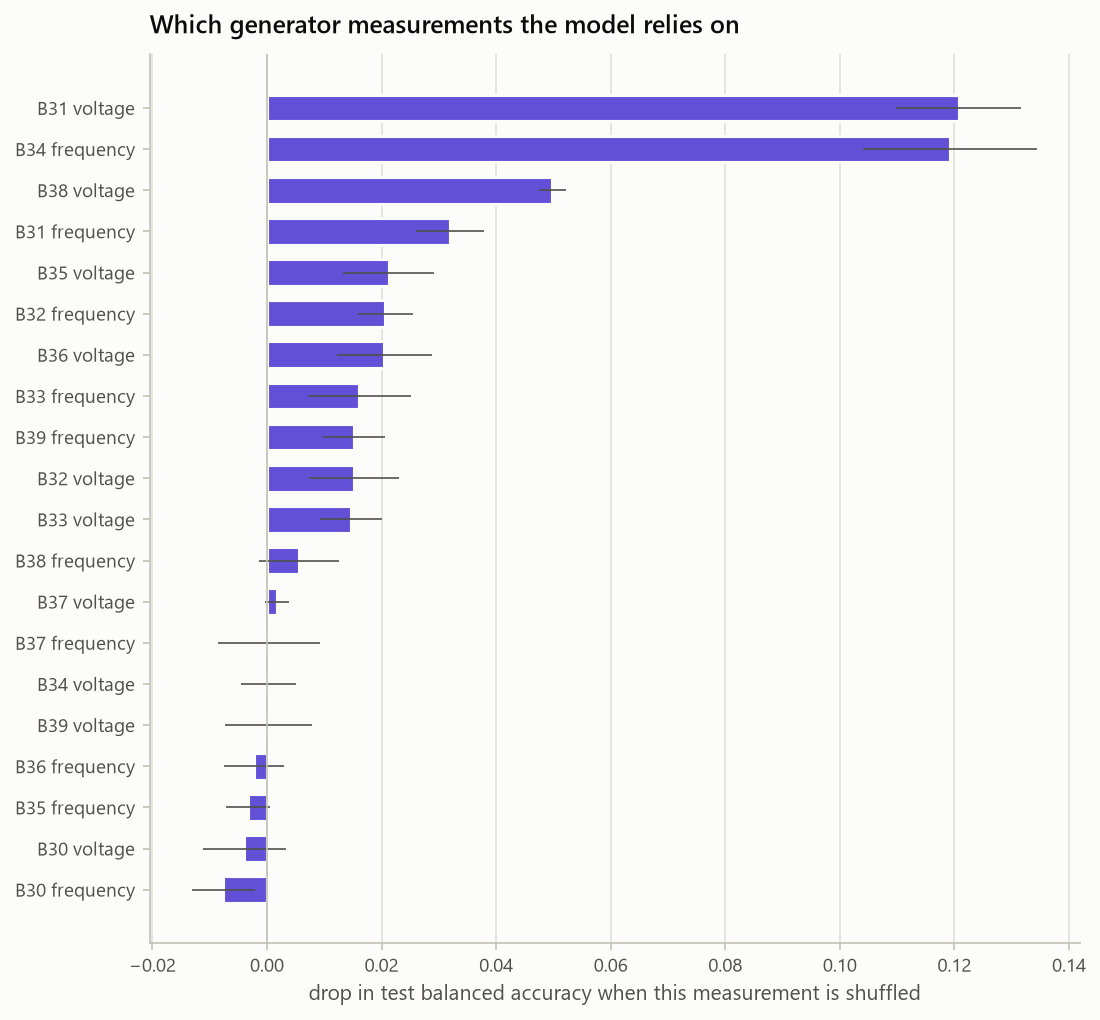
\includegraphics[width=0.75\linewidth]{19_feature_importance.png}
  \caption{Permutation importance of each bus voltage and frequency (mean $\pm$ standard deviation over ten
  repetitions).}
  \label{fig:importance}
\end{figure}

%=====================================================================================
\section{Discussion}
%=====================================================================================
\paragraph{Accuracy and its uncertainty.} The three estimates (cross-validation 0.974, validation 0.961, test 0.955)
differ by up to two points because each hold-out set contains only about 106 contingencies and the errors are
concentrated in a handful of them. In particular, the test set happens to contain the Bus~38 generator trip and the
line 22--23 trip, which alone cause ten false alarms. The cross-validated mean and spread is the steadiest estimate;
a realistic expectation for unseen contingencies of the simulated kinds is a balanced accuracy of about 0.95--0.97.

\paragraph{Grouped splitting matters.} Splitting by contingency prevents the five near-identical load-level variants of a
contingency from appearing in both training and test data. The results therefore describe the more demanding and more
realistic task of assessing a contingency the model has never seen.

\paragraph{Impossible readings.} The ten impossible rows were kept and used for training. With them in the training
data, cross-validation prefers the robust scaler (median and interquartile range, then clipping), whose scale is not
distorted by the extreme values; the standard scaler is only slightly behind. Because all ten rows are clearly unstable,
their effect on accuracy is small. Their real influence is on how the model treats inputs far outside the normal range,
which the next experiment will examine by removing or capping them on the same validation and test sets.

\paragraph{Inputs outside the training range.} An RBF-kernel SVM can only interpolate between the cases it has seen.
Inputs outside the training range, such as the B38 frequency after the Bus~38 generator trip, are extrapolations and
are the most likely to be misclassified. The prediction tool reports such inputs with every prediction. In the test set,
32 cases had at least one input outside the training range; 5 of them were misclassified, all from the Bus~38 trip.

\paragraph{Limitations.} Only ten generator-trip contingencies exist, so the model has seen very few examples of this
kind. The four samples cover only the early post-disturbance period, so instability that develops later leaves little
trace in them (for example the short three-phase fault on line 16--19 missed in the validation set). All results refer
to simulated data of one test system and one set of operating conditions.

%=====================================================================================
\section{Conclusions and future work}
\label{sec:future}
%=====================================================================================
An RBF-kernel SVM using only four voltage and four frequency samples from each of the ten generators predicts the
transient stability of the IEEE 39-bus system with a balanced accuracy of about 0.96--0.97 on contingencies it has not
seen (cross-validation 0.974, validation 0.961, test 0.955) and found 93 of 97 unstable test cases. The procedure
(grouped split, cross-validated hyperparameter selection, a single final test) gives an honest estimate of this
performance. Planned next steps:
\begin{enumerate}
  \item \textbf{Second experiment on outliers:} remove or cap the impossible readings, and compare with this baseline on
        the same validation and test sets.
  \item \textbf{More diverse scenarios}, especially generator trips and additional fault locations.
  \item \textbf{Decision threshold:} shift the boundary of the instability score to trade false alarms for fewer missed
        unstable cases.
  \item \textbf{Engineered features}, e.g.\ the frequency spread between generators, which on its own separates the
        classes well.
  \item \textbf{Benchmark models} (e.g.\ gradient boosting, neural networks) on the same split.
\end{enumerate}

\appendix
%=====================================================================================
\section{Software implementation}
%=====================================================================================
\subsection{Project structure}
The analysis is implemented in Python 3 with scikit-learn 1.9, pandas and matplotlib.
\begin{lstlisting}[language={},numbers=none,caption={Project folder.}]
Data Anltics/
|-- IEEE39_voltage_frequency_4sample_SVM_dataset.csv
|-- transient_stability_svm.ipynb   notebook: complete analysis with all graphs
|-- train_model.py                  command-line training (same steps as the notebook)
|-- predict.py                      command-line prediction for new cases
|-- requirements.txt
|-- stability_svm/                  Python package
|   |-- config.py     file paths, feature names, split sizes, tuning grid
|   |-- data.py       loading, quality checks, train/validation/test split
|   |-- model.py      SVM pipeline, cross-validated tuning, save/load
|   |-- evaluate.py   metrics, breakdowns, permutation importance, learning curve
|   |-- plots.py      all figures
|   |-- predict.py    predictions for new cases
|-- models/stability_svm.joblib     trained model
|-- figures/                        all figures (PNG)
|-- reports/                        text report, tuning grids, test predictions
|-- examples/                       example input files for predict.py
|-- report/                         this LaTeX report
\end{lstlisting}

\begin{lstlisting}[language={},numbers=none,caption={Installing and running.}]
py -m pip install -r requirements.txt
py train_model.py                                  # train, evaluate, save results
py predict.py examples\example_case_unstable.csv   # predict one case
\end{lstlisting}

\subsection{Key code}
\begin{lstlisting}[caption={Split by contingency into training, validation and test sets (\code{data.py}).}]
def _group_split(df, fraction, seed):
    """Hold out about `fraction` of the contingencies, keeping the unstable share similar."""
    n_splits = max(2, round(1 / fraction))
    splitter = StratifiedGroupKFold(n_splits=n_splits, shuffle=True, random_state=seed)
    keep_idx, hold_idx = next(splitter.split(df, df[LABEL], df[GROUP]))   # GROUP = "Contingency_ID"
    return df.iloc[keep_idx], df.iloc[hold_idx]


def split_train_val_test(df, test_fraction=0.15, val_fraction=0.15, seed=42, extremes_in_train=True):
    # contingencies with impossible readings always go to the training set
    forced_ids = set(df.loc[extreme_rows(df), GROUP]) if extremes_in_train else set()
    pool = df[~df[GROUP].isin(forced_ids)]
    rest, test = _group_split(pool, test_fraction, seed)
    train, val = _group_split(rest, val_fraction / (1 - test_fraction), seed + 1)
    train = pd.concat([train, df[df[GROUP].isin(forced_ids)]])
    return train, val, test
\end{lstlisting}

\begin{lstlisting}[caption={Scaler and RBF-kernel SVM in one pipeline (\code{model.py}).}]
def build_model(scaler="robust_clip", C=10.0, gamma="scale"):
    if scaler == "standard":
        steps = [("scale", StandardScaler())]
    elif scaler == "robust_clip":
        steps = [("scale", RobustScaler()),
                 ("clip", FunctionTransformer(np.clip, kw_args={"a_min": -20, "a_max": 20}))]
    steps.append(("svm", SVC(kernel="rbf", C=C, gamma=gamma, class_weight="balanced")))
    return Pipeline(steps)


def instability_score(model, X):
    """Signed distance from the SVM boundary, > 0 means Unstable."""
    d = model.decision_function(X)          # > 0 points to model.classes_[1]
    return -d if model.classes_[1] == STABLE else d
\end{lstlisting}

\begin{lstlisting}[caption={Hyperparameter selection by grouped five-fold cross-validation inside the training set (\code{model.py}).}]
def tune_with_cv(X_train, y_train, groups, grid=PARAM_GRID, n_splits=5, seed=42):
    rows = []
    for scaler in grid["scaler"]:
        search = GridSearchCV(build_model(scaler=scaler),
                              {"svm__C": grid["C"], "svm__gamma": grid["gamma"]},
                              cv=StratifiedGroupKFold(n_splits, shuffle=True, random_state=seed),
                              scoring="balanced_accuracy", n_jobs=-1)
        search.fit(X_train, y_train, groups=groups)
        r = search.cv_results_
        for i, p in enumerate(r["params"]):
            rows.append({"scaler": scaler, "C": p["svm__C"], "gamma": p["svm__gamma"],
                         "cv_bal_acc": r["mean_test_score"][i], "cv_std": r["std_test_score"][i]})
    res = pd.DataFrame(rows).sort_values(["cv_bal_acc", "cv_std"], ascending=[False, True])
    best = res.iloc[0]
    return res, {"scaler": best["scaler"], "C": float(best["C"]), "gamma": best["gamma"]}
\end{lstlisting}

\begin{lstlisting}[caption={Complete training and evaluation procedure (\code{train\_model.py} and the notebook).}]
df = data.add_scenario_details(data.load_dataset())        # all 3,715 cases, nothing removed
train, val, test = data.split_train_val_test(df)           # grouped by Contingency_ID
X_tr, y_tr = data.get_xy(train)                            # the 80 measurements and the label

# 1. choose scaler, C and gamma inside the training set
cv_results, best = model.tune_with_cv(X_tr, y_tr, train["Contingency_ID"])

# 2. independent check on the validation set
selection_model = model.build_model(**best).fit(X_tr, y_tr)
val_pred, val_score, m_val = evaluate.evaluate(selection_model, val)

# 3. final model on training + validation data, evaluated once on the test set
trainval = pd.concat([train, val])
final = model.build_model(**best).fit(*data.get_xy(trainval))
test_pred, test_score, m_test = evaluate.evaluate(final, test)

model.save_model(final, best, {"validation": m_val, "test": m_test}, trainval)
\end{lstlisting}

\begin{lstlisting}[caption={Metrics with the unstable class as the positive class (\code{evaluate.py}).}]
def classification_metrics(y_true, y_pred, score=None):
    m = {
        "accuracy": accuracy_score(y_true, y_pred),
        "balanced_accuracy": balanced_accuracy_score(y_true, y_pred),
        "unstable_recall": recall_score(y_true, y_pred, pos_label=UNSTABLE),
        "unstable_precision": precision_score(y_true, y_pred, pos_label=UNSTABLE),
        "stable_recall": recall_score(y_true, y_pred, pos_label=STABLE),
    }
    if score is not None:                                   # instability score, > 0 = unstable
        is_unstable = np.asarray(y_true) == UNSTABLE
        m["roc_auc"] = roc_auc_score(is_unstable, score)
        m["average_precision"] = average_precision_score(is_unstable, score)
    return m
\end{lstlisting}

\begin{lstlisting}[caption={Predicting a new case from the $10 \times 4$ voltage and frequency samples (\code{predict.py}).}]
from stability_svm.predict import predict_case

# rows: generators B30 ... B39, columns: samples 1 ... 4
vmag = [[...], ...]     # 10 x 4 voltage magnitudes (p.u.)
freq = [[...], ...]     # 10 x 4 frequencies (Hz)

result = predict_case(vmag, freq)
# result["prediction"]             -> "Stable" or "Unstable"
# result["instability_score"]      -> float, > 0 means unstable
# result["outside_training_range"] -> inputs outside the range seen in training
\end{lstlisting}

%=====================================================================================
\section{Cross-validation results}
\label{app:grid}
%=====================================================================================
\begin{table}[htbp]
\centering
\caption{The ten best settings in grouped five-fold cross-validation on the training set.}
\label{tab:cvtop}
\begin{tabular}{rllrr}
\toprule
Rank & Scaler & $C$ / $\gamma$ & Balanced accuracy & Std.\ dev. \\
\midrule
1  & robust + clip & 10 / 0.001   & \textbf{0.9743} & 0.0159 \\
2  & robust + clip & 10 / 0.01    & 0.9737 & 0.0182 \\
3  & robust + clip & 1 / 0.01     & 0.9730 & 0.0156 \\
4  & standard      & 100 / 0.001  & 0.9715 & 0.0128 \\
5  & standard      & 10 / 0.003   & 0.9714 & 0.0151 \\
6  & robust + clip & 10 / 0.003   & 0.9703 & 0.0144 \\
7  & robust + clip & 100 / 0.001  & 0.9675 & 0.0169 \\
8  & robust + clip & 1 / scale    & 0.9673 & 0.0196 \\
9  & robust + clip & 1000 / 0.03  & 0.9670 & 0.0305 \\
10 & robust + clip & 10 / scale   & 0.9660 & 0.0184 \\
\bottomrule
\end{tabular}
\end{table}

\end{document}
